\documentclass[a4paper,12pt,twoside]{article}

%PACKAGES

\usepackage[T1]{fontenc}
\usepackage{lmodern}

\usepackage[utf8]{inputenc}
\usepackage[slovak]{babel}
\usepackage{comment}

\usepackage{graphicx,amsmath,amssymb, amsthm, multicol}
\usepackage{pdfpages}

\usepackage[nottoc]{tocbibind}
\usepackage{mathrsfs}
\usepackage{psfrag}
\usepackage[small,bf]{caption}
\usepackage{ifthen}

\usepackage{xcolor}
\usepackage{listings}
\usepackage{enumitem}

\usepackage[toc,page]{appendix}

\usepackage{url}
\urlstyle{rm}
\renewcommand\UrlFont{\color{black}}

\usepackage{pgfplots}

\usepackage{tikz}
\usetikzlibrary{positioning,chains,fit,shapes,calc}

% \renewcommand{\familydefault}{\rmdefault}

\newtheorem{defin}{Definícia}[section]
\newtheorem{theorem}[defin]{Veta}
\newtheorem{prop}[defin]{Tvrdenie}
\newtheorem{lema}[defin]{Lema}
\newtheorem{cor}[defin]{Dôsledok}
\newtheorem{hypoteza}{Hypotéza}[section]
\newtheoremstyle{comment}{}{}{}{}{}{:}{ }{#1}
\theoremstyle{comment}
\newtheorem{dokaz}{Dôkaz}[section]
\newtheorem{com}{\textit{Poznámka}}

\usepackage{hyperref}                                     
\hypersetup{%  http://www.tug.org/applications/hyperref/
bookmarksnumbered,
pdfstartview={FitH},
linkcolor=black,
citecolor=black,
colorlinks=true,
pdfpagemode={None},
plainpages=false
}%

%%\usepackage{fullpage}
%%\setlength{\topmargin}{-0.5cm}
%%\setlength{\headheight}{0cm}
%%\setlength{\headsep}{0in}
\setlength{\textheight}{24cm}
\setlength{\textwidth}{15.5cm}
\addtolength{\voffset}{-1.2cm}
\addtolength{\hoffset}{-0.3cm}
%%\addtolength{\rightmargin}{-1cm}
\setlength{\parindent}{0.5cm}
\setlength{\parskip}{0in}
\linespread{1.5}

\setcounter{MaxMatrixCols}{20}

\begin{document}

  \thispagestyle{empty}
\begin{center}
{\large \bf UNIVERZITA KOMENSKÉHO V BRATISLAVE \\
FAKULTA MATEMATIKY, FYZIKY A INFORMATIKY}
\end{center}
%\begin{titlepage}
%    \rmfamily
%    \begin{center}
%      \LARGE\scshape
%      \theuniversity\\
%      \Large\upshape
%      \thefaculty\\
%      \large
%      \thedepartment
%    \end{center}
%

\vspace{2cm}
\begin{figure}[!h]
   \centering
     %
\includegraphics[width=3.5cm]{logoUK.jpg}
\end{figure}

\vspace{1cm}
\begin{center}
{\large \bf Predikcia bankrotu firiem v slovenskom prostredí \\
\vspace{3cm}
DIPLOMOVÁ PRÁCA}
\end{center}

\vfill
%
\begin{multicols}{2}
{\bf
\begin{flushleft} 2022 \end{flushleft}
\begin{flushright} Bc. Róbert Druska \end{flushright} 
}
\end{multicols}


  \newpage
\thispagestyle{empty}
\begin{center}
{\large UNIVERZITA KOMENSKÉHO V BRATISLAVE \\
FAKULTA MATEMATIKY, FYZIKY A INFORMATIKY}
\end{center}


\vspace{5cm}
\begin{center}
{\large \bf Predikcia úpadku slovenských firiem \\
\vspace{3cm}
DIPLOMOVÁ PRÁCA}
\end{center}

\vfill
\begin{flushleft}
\begin{tabular}{ll}
Študijný program: & Pravdepodobnosť a matematická štatistika \\
Študijný odbor: & Aplikovaná matematika \\
Školiace pracovisko: & Katedra aplikovanej matematiky a štatistiky \\
Vedúci práce: & doc. Mgr. Radoslav Harman, PhD. \\
\end{tabular}
\end{flushleft}

\vfill
%
\begin{multicols}{2}
\begin{flushleft} Bratislava 2022 \end{flushleft}
\begin{flushright} {\bf Bc. Róbert Druska} \end{flushright}
\end{multicols}



%   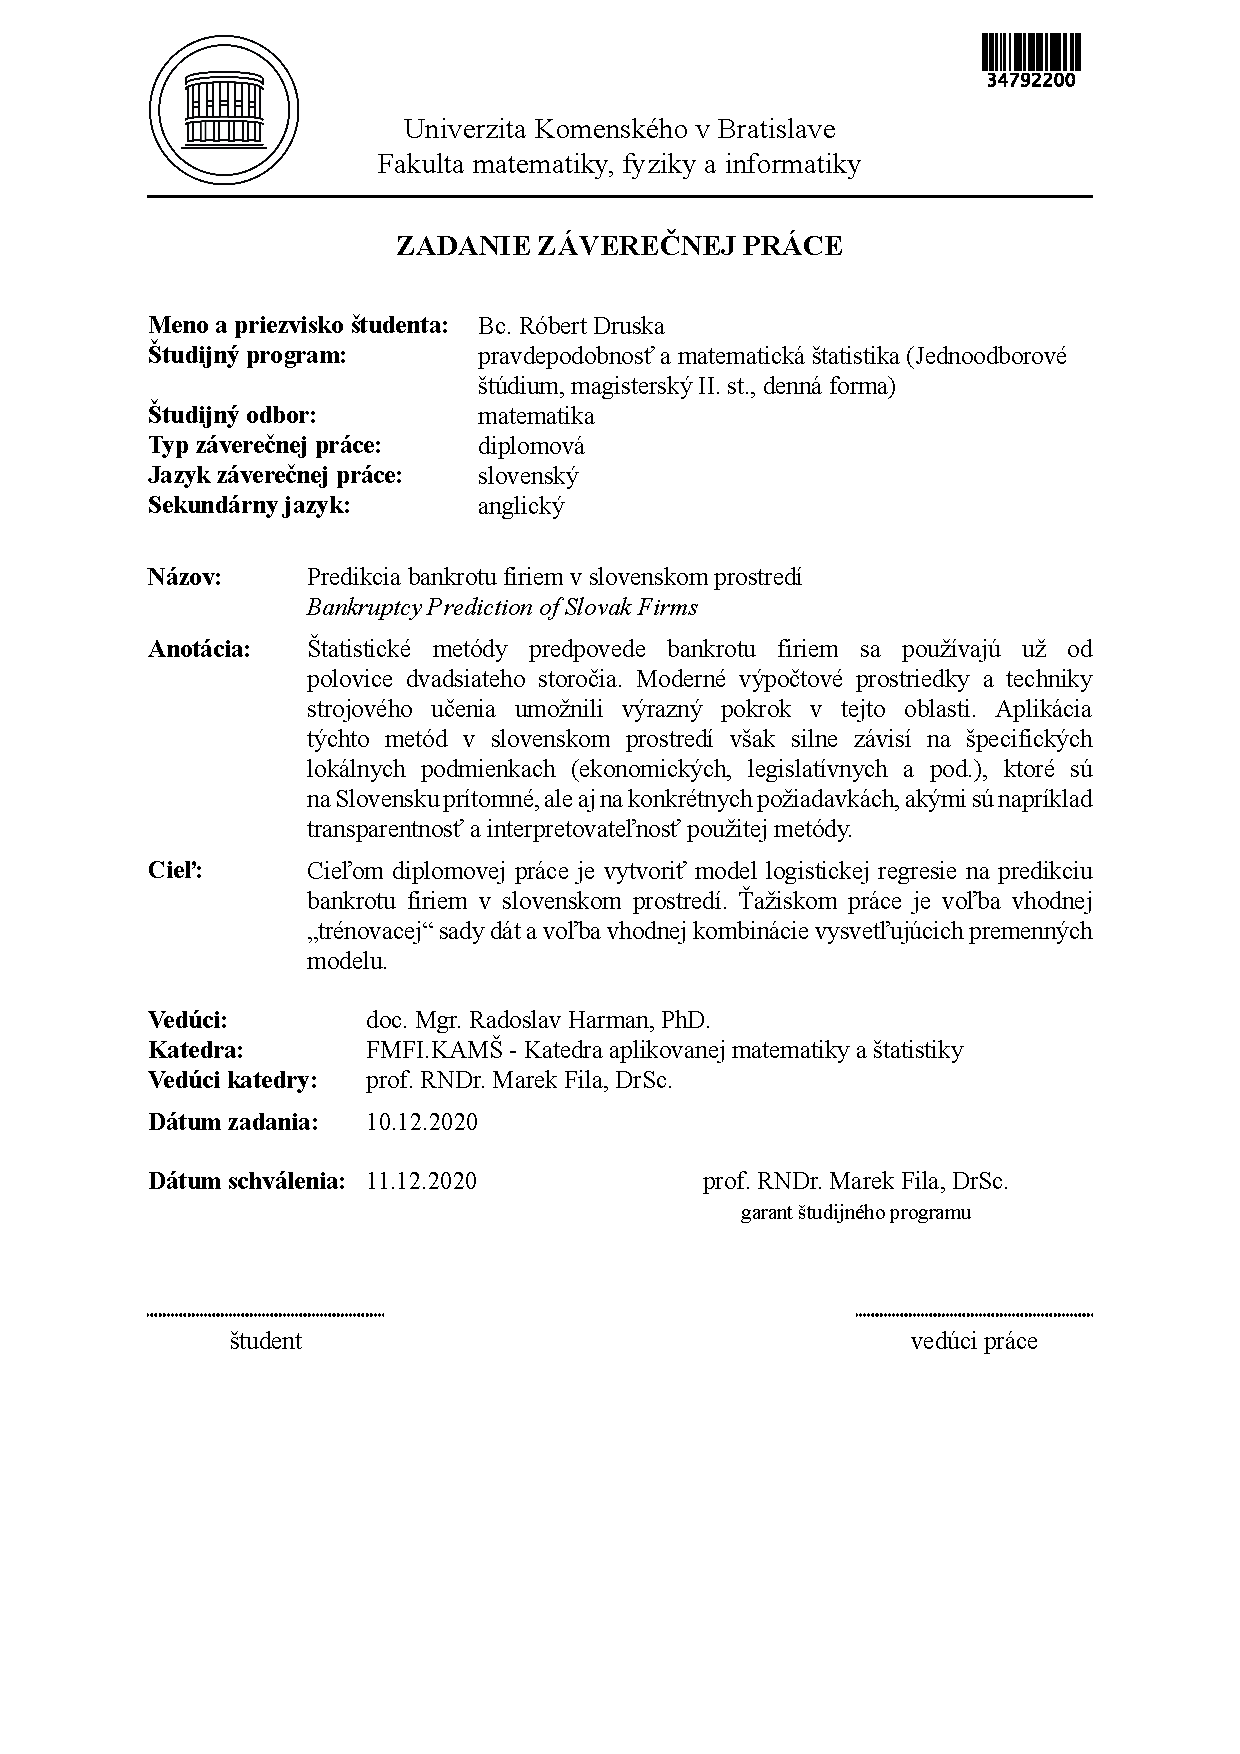
\includepdf[pages={1}, offset=25 -75]{zadanieRD.pdf}

  

\vglue0pt
\vfill
\thispagestyle{empty}
\paragraph{Poďakovanie}

Touto cestou by som sa chcel poďakovať svojmu školiteľovi, Radoslavovi Harmanovi, za jeho ochotu a množstvo dobrých a pravidelných rád pri písaní tejto práce.
Ďakujem tiež svojej kolegyni Monike Hrnčárovej za cenné analýzy predchádzajúce praktickým častiam práce, a svojej mame za gramatickú a štylistickú korektúru.
V neposlednom rade ďakujem svojim priateľom za oporu v posledných mesiacoch písania.


  \newpage
  \thispagestyle{empty}
\section*{Abstrakt}
DRUSKA, Róbert: Predikcia úpadku slovenských firiem [Diplomová práca],
Univerzita Komenského v Bratislave,
Fakulta matematiky, fyziky a informatiky,
Katedra aplikovanej matematiky a štatistiky,
školiteľ: doc. Mgr. Radoslav Harman, PhD.,
Bratislava, 2020, TODO s.

TODO Lorem ipsum dolor sit amet, consectetur adipiscing elit, sed do eiusmod tempor incididunt ut labore et dolore magna aliqua. Ut enim ad minim veniam, quis nostrud exercitation ullamco laboris nisi ut aliquip ex ea commodo consequat. Duis aute irure dolor in reprehenderit in voluptate velit esse cillum dolore eu fugiat nulla pariatur. Excepteur sint occaecat cupidatat non proident, sunt in culpa qui officia deserunt mollit anim id est laborum.

\begin{flushleft}
  \textbf{Kľúčové slová:} logistická regresia, TODO
\end{flushleft}

  \newpage
  \thispagestyle{empty}
\section*{Abstract}
DRUSKA, Róbert: Bankruptcy prediction [Master thesis],
Comenius University in Bratislava,
Faculty of Mathematics, Physics and Informatics,
Department of Applied Mathematics and Statistics,
supervisor: doc. Mgr. Radoslav Harman, PhD.,
Bratislava, 2020, TODO p.

TODO Lorem ipsum dolor sit amet, consectetur adipiscing elit, sed do eiusmod tempor incididunt ut labore et dolore magna aliqua. Ut enim ad minim veniam, quis nostrud exercitation ullamco laboris nisi ut aliquip ex ea commodo consequat. Duis aute irure dolor in reprehenderit in voluptate velit esse cillum dolore eu fugiat nulla pariatur. Excepteur sint occaecat cupidatat non proident, sunt in culpa qui officia deserunt mollit anim id est laborum.

\begin{flushleft}
  \textbf{Keywords:} logistic regression, TODO
\end{flushleft}
  \newpage \tableofcontents
  \setcounter{page}{7}
 % \newpage
 % \listoffigures
 % \newpage
 % \listoftables  
  \newpage

    \section*{Úvod}	          
    \markboth{ÚVOD}{ÚVOD}  
    \addcontentsline{toc}{section}{Úvod}
    
    Predikcia bankrotu firiem je predmetom akademického aj profesionálneho výskumu už po dlhé desaťročia.
Motivácia stojaca za hľadaním modelov na predikciu úpadku firiem je rôzna.
Prvé modely vytvorené na základe dát o verejne obchodovateľných spoločnostiach v USA
boli využívané pri analýzach predchádzajúcich nákupom akcií \cite{altman1968}.
Modely kreditného rizika našli veľké využitie v bankovníctve – banky a iné finančné inštitúcie disponujú internými modelmi,
ktorými vyhodnocujú finančnú kondíciu svojich klientov a ich hodnotenia využívajú napr. pri stanovovaní úrokových sadzieb.
Takisto aj súkromné spoločnosti a živnostníci môžu využiť modely kreditného rizika pri bežnom vykonávaní svojej podnikateľskej praxe.

V prvých dvoch kapitolách sa oboznamujeme s problematikou bankrotu na Slovenku a predstavíme si dva známe modely kreditného rizika – Altmanovo Z-skóre a český index IN05.
Tretia kapitola je teoretickou predprípravou k metodike,
ktorú sme v práci použili na modelovanie predikcie bankrotu v slovenskom prostredí.
Oboznámime sa v nej s logistickou regresiou a tiež s metódou \emph{BACE}, ktorá slúži na výber vhodnej kombinácie parametrov do modelu.
V štvrtej kapitole sa bližšie venujeme metodike praktickej časti práce.

V piatej kapitole dôkladne opíšeme proces vytvorenia modelov predikcie bankrotu
od popisu dát cez technické detaily modelovania až po porovnanie nami vytvorených modelov s Altmanovým Z-skóre a indexom IN05
aj medzi sebou navzájom. Posledná, šiesta kapitola obsahuje diskusiu o interpretácii výstupov bankrotových modelov. 

  \newpage
  \section{Bankrot na Slovensku}
\label{bankruptcy}

Cieľom tejto práce je vytvoriť model na predikciu úpadku firiem na základe jej finančných údajov.
Pre účely modelovania si na začiatok zadefinujme, čo budeme rozumieť pod pojmom úpadok.
Problematikou bankrotu právnických a fyzických osôb na Slovensku sa venuje najmä zákon 7/2005 Z. z. o konkurze a reštrukuturalizácii \cite{zbierkazakonov},
ktorý definuje úpadok nasledovne.

\bigskip
\textit{(1)
Dlžník je v úpadku, ak je platobne neschopný alebo predlžený. Ak dlžník podá návrh na vyhlásenie konkurzu, predpokladá sa, že je v úpadku.}

\textit{(2)
Právnická osoba je platobne neschopná, ak nie je schopná plniť 30 dní po lehote splatnosti aspoň dva peňažné záväzky viac ako jednému veriteľovi. […]}

\textit{(3)
Predlžený je ten, kto je povinný viesť účtovníctvo podľa osobitného predpisu, má viac ako jedného veriteľa a hodnota jeho záväzkov presahuje hodnotu jeho majetku. […]}
\bigskip

Keď je právnická osoba v úpadku, je potrebné vyhlásiť konkurz alebo reštrukturalizáciu.
Konkurzné a reštrukturalizačné konania schvaľuje súd, vďaka čomu poznáme presný dátum ich začiatku, čo sa nám zíde pri modelovaní.

Konkurz znamená speňaženie majetkovej podstaty dlžníka a pomerné uspokojenie jeho veriteľov z tohto majetku.
Konkurz má charakter likvidačného konania a jeho výsledkom je zrušenie a zánik podniku.
V bežnej praxi ide o zdĺhavý proces, ktorý môže trvať aj niekoľko rokov.

Na rozdiel od konkurzu reštrukturalizácia nemá likvidačný charakter a je možné vyhlásiť ju už v čase hroziaceho úpadku.
Cieľom reštrukturalizácie je zachovanie podniku alebo jeho časti a postupné uspokojenie veriteľov spôsobom dohodnutým v reštrukturalizačnom pláne.
Uspokojenie pohľadávok býva v praxi rýchlejšie ako pri konkurze.
V prípade, že reštrukturalizácia bude úspešná, právnická osoba može naďalej pokračovať v podnikateľskej činnosti,
avšak predpokladom jej úspechu je to, že pohľadávky veriteľov sa budú počas ďalšieho fungovania podniku uspokojovať vo vyššej miere ako v prípade konkurzu.

Spoločným znakom konkurzu a reštrukturalizácie je skutočnosť, že dlžník sa nachádza v krízovej ekonomickej situácii.
Pre účely tejto práce budeme \emph{bankrotom} rozumieť začiatok konkurzného alebo reštrukturalizačného konania.

\subsection{Bankrot - vzácna udalosť}

Úpadok alebo bankrot možno považovať v rámci populácie aktívnych firiem za vzácnu udalosť.
Databáza \emph{FinStat}, ktorej dáta budeme využívať v tejto práci, eviduje celkovo 6946 prípadov konkurzného alebo reštrukturalizačného konania za obdobie existencie samostatnej Slovenskej republiky.
Ako uvidíme, nie každé z týchto konaní sa hodí na modelovanie, či už kvôli nedostatku dostupných dát alebo inej príčiny.

Napríklad, z počtu 6946 firiem v úpadku len pre 3730 firiem poznáme presný dátum začiatku konkurzného alebo reštrukturalizačného konania.
Dátum začiatku konania nepoznáme zväčša pre staršie firmy, ktoré zanikli pred rokom 2010, a pre ktoré by sme v mnohých prípadoch aj tak nemali dostatok dát pre úspešné zahrnutie do modelu.

V tabuľke uvádzame počet konkurzov a reštrukturalizácií a počet aktívnych firiem od roku 2011 po rok 2020.

\begin{center}
    \begin{tabular}{ |c|c|c|c|p{3cm}|p{3cm}| }
        \hline
        Rok & Konkurzy & Reštrukturalizácie & Spolu & Celkový počet aktívnych firiem & Proporcia firiem v úpadku \\
        \hline
        2011 & 282 & 21 & 303 & TODO & TODO \\
        \hline
        2012 & 296 & 36 & 332 & & \\
        \hline
        2013 & 318 & 49 & 367 & & \\
        \hline
        2014 & 329 & 56 & 385 & & \\
        \hline
        2015 & 325 & 49 & 374 & & \\
        \hline
        2016 & 222 & 35 & 257 & & \\
        \hline
        2017 & 215 & 22 & 237 & & \\
        \hline
        2018 & 256 & 6 & 262 & & \\
        \hline
        2019 & 254 & 8 & 262 & & \\
        % pozn: v roku 2019 mala jedna firma konanie s kategoriou "ine", ide o firmu s ico 36595098 ... po rucnej kontrole som ju zaradil medzi restrukturalizacie
        \hline
        2020 & 185 & 19 & 204 & & \\
        \hline
    \end{tabular}
\end{center}
\bigskip

Ako vidíme, počet firiem v úpadku sa každoročne nachádza pod hranicou 0,5 \% z aktívnych firiem.
Z uvedeného vyplýva, že pri modelovaní úpadku firiem budeme pracovať so silno nevyváženými dátami (angl. \emph{angl. unbalanced classes}).
Napriek tomu, že bankrot je v populácii firiem vzácny, ide o udalosť, ktorej predpovedanie je zaujímavé pre množstvo strán -
napr. pre manažment firiem, majiteľov firemného kapitálu, poskytovateľov pôžičiek, investorov či poisťovateľov.

TODO: bližší opis bankrotov podľa odvetví, veľkosti firiem, potenciálne niečo o vplyve covid pandémie atď. a pod.,
dá sa tu spraviť veľa deskriptívnej štatistiky

%   \newpage  
% 	\section{Teoretická predpríprava}
\label{teoreticka predpriprava}

\subsection{Logistická regresia}
 
Logistická regresia je štatistická metóda využívaná pri binárnej klasifikácii.
Cieľom logistickej regresie je modelovať pravdepodobnosť nejakej triedy alebo udalosti (vysvetľovanej premennej)
na základe jednej alebo viacerých vysvetľujúcich premenných. TODO

Pred tým, než opíšeme, ako presne logistická regresia funguje, si zadefinujme niekoľko dôležitých pojmov, s ktorými logistická regresia narába.

\begin{defin}
    Logistická funkcia \( \sigma : \mathbb{R} \rightarrow (0, 1) \) je definovaná ako:
    \[
        \sigma(t) = \frac{e^t}{e^t + 1} = \frac{1}{1 + e^{-t}}
    \]
    Inverzná funkcia k logistickej sa nazýva logit funkcia a spĺňa:
    \[
        logit(t) = \sigma^{-1}(t) = \ln\left(\frac{p}{1 - p}\right)
    \]
    pre \( p \in (0, 1) \).
\end{defin}

Na obrázku je zobrazený graf logistickej funkcie na intervale \( (-6, 6) \):

% \begin{center}
%     \begin{tikzpicture}
%     \begin{axis}[
%         xlabel={x},
%         ylabel={y},
%         xmin=-6, xmax=6,
%         ymin=0, ymax=1,
%         xtick={-4,-2,0,2,4},
%         ytick={0,0.2,0.4,0.6,0.8,1},
%         legend pos=north west,
%         ymajorgrids=true,
%         grid style=dashed,
%         height=8cm,
%         width=15cm,
%     ]
    
%     \addplot[
%         color=blue,
%         mark=square,
%         ]
%         coordinates {
%         (2, 1.0)(3, 0.5)(4, 0.25)(5, 0.16667)(6, 0.11111)(7, 0.08333)(8, 0.0625)(9, 0.05)(10, 0.04)(11, 0.03333)(12, 0.02778)(13, 0.02381)(14, 0.02041)(15, 0.01786)(16, 0.015625)
%         };
%         % \legend{Rozptyl}
        
%     \end{axis}
%     \end{tikzpicture}
% \end{center}


\begin{center}
\begin{tikzpicture}[>=stealth]
    \begin{axis}[
        xmin=-6,xmax=6,
        ymin=0,ymax=1,
        axis x line=middle,
        axis y line=middle,
        axis line style=<->,
        xlabel={$x$},
        ylabel={$y$},
        ]
        \addplot[no marks,blue,solid] expression[domain=-6:6,samples=100]{1/(1 + exp(-x))};
    \end{axis}
\end{tikzpicture}
\end{center}

Argumentom prirodzeného logaritmu v logit funkcii je výraz \( \frac{p}{1 - p} \) pre \( p \in (0, 1) \).
Ak takéto \(p\) budeme chápať ako pravdepodobnosť, výraz \( \frac{p}{1 - p} \) predstavuje takzvaný pomer šancí (\emph{angl. odds-ratio}).
Napríklad pri hode kockou je pravdepodobnosť padnutia šestky rovná \( 1/6 \) a pomer šancí je \( \frac{\frac{1}{6}}{1 - \frac{1}{6}} = \frac{\frac{1}{6}}{\frac{5}{6}} = \frac{1}{5} = 1 : 5\),
čo znamená, že 1 možný výsledok hodu kockou zodpovedá šestke a 5 možných výsledkov šestke nezodpovedá.

Nech \( Y \) je binárna vysvetľovaná premenná, ktorej zodpovedá vektor vysvetľujúcich premenných \( x = (x_1, x_2, \ldots, x_k) \).
Pre \( Y \) zjavne platí \( P(Y = 1|x) = 1 - P(Y = 0|x) \).
Logistická regresia predpokladá, že logaritmus pomeru šancí (\emph{angl. log-likelihood ratio}) možno modelovať ako lineárnu funkciu zložiek vektora \( x \).

\[
\ln \left( \frac{P(Y = 1|x)}{P(Y = 0|x)} \right) = \ln \left( \frac{P(Y = 1|x)}{1 - P(Y = 1|x)} \right) = \beta_0 + \beta^T x
\]

Po úpravách sa ľahko dopracujeme k záveru, že pravdepodobnosť \( P(Y = 1|x) \) je rovná výstupu logistickej funkcie, ktorej argument bude hľadaná lineárna kombinácia zložiek vektora \( x \).

\begin{equation} \label{logistic_regression}
P(Y = 1|x) = \frac{1}{1 - e^{-(\beta_0 + \beta^T x})} := h(x)
\end{equation}

Ak logistickú regresiu používame na predikciu (čo budeme robiť neskôr v tejto práci),
vzorec (\ref{logistic_regression}) nám poslúži na výpočet pravdepodobnosti \( P(Y = 1|x) \) pri danom novom \( x \).

\subsubsection{Odhad parametrov v logistickej regresii}

Majme teda zovšebecnený regresný model tvaru

\[
h_\beta(x) = P(Y = 1|x) = \frac{1}{1 - e^{-(\beta_0 + \beta^T x})}
\]

Neznámymi parametrami v tomto modeli sú regresory \( \beta = (\beta_1, \ldots, \beta_k) \).
Na odhad regresných koeficientov sa vo väčšine prípadov používa metóda maximálnej vierohodnosti.
Na rozdiel od obyčajnej lineárnej regresie s normálne rozdelenými chybami, v logistickej regresii nie je možné nájsť exaktné vyjadrenie parametrov \( \beta \),
a na ich odhad sa používa nejaká iteračná metóda.

Keďže \(Y\) nadobúda len hodnoty z \( \{0, 1\} \), pre distribučnú funkciu \(Y\) platí:

\[
P(y | x; \beta ) = h_\beta(x)^y (1 - h_\beta(x))^{1 - y}
\]

Majme namerané vektory dát \( x_1, \ldots, x_n \), \( x_i = x_{i1}, \ldots, x_{ik} \),
a k nim prislúchajúce \( y_1, \ldots, y_n \). Potom pre funkciu vierohodnosti parametra \( \beta \) platí

\[
L(\beta | y; ) TODO
\]

Trénovanie logistickej regresie spočíva v maximalizovaní funkcie vierohodnosti,
čo je ekvivalentné maximalizácii jej logaritmu (\emph{angl. log-likelihood function}), a teda hľadáme

\[
TODO
\]

Na nájdenie maxima log-likelihood funkcie sa používajú iteračné metódy,
napr. funkcia \emph{glm} v základnej verzii jazyka \emph{R} využíva metódu \emph{IRLS} (\emph{iteratively reweighted least squares}).

\subsubsection{Sumárne štatistiky v logistickej regresii}

TODO: Tu napíšem niečo o hodnotách ako \(R^2\) atď., ešte to nemám celkom premyslené.

\subsubsection{Interpretácia parametrov v logistickej regresii}

%   \newpage
% 	\input{09 kap3}

%   \newpage
%   \input{10 kap4}

	\newpage
  \section*{Záver}
    \addcontentsline{toc}{section}{Záver}
    \markboth{ZÁVER}{ZÁVER} 
    TODO
  
  \newpage
  \renewcommand{\refname}{Zoznam použitej literatúry}
  \begin{thebibliography}{99}

	% \bibitem{pazman} Pázman, A., Lacko, V.: {\it Prednášky z regresných modelov}, Vydavateľstvo UK, Bratislava, 2012, 2015

	% \bibitem{kniha} Freedman, David: {\it Statistical models: Theory and practice}, Cambridge University Press, New York, 2005

	% \bibitem{kniha} Rencher, Alvin C.: {\it Methods of Multivariate Analysis}, John Wiley \& Sons, New York, 2002

	% \bibitem{yan} Yan, Xin: {\it Linear Regression Analysis: Theory and Computing}, World Scientific Publishing Co. Pte. Ltd., Singapore, 2009

	% \bibitem{kniha} \url{http://oeis.org/A002724}

	% \bibitem{cheng} Cheng, C.S.: {\it Maximizing the total number of spanning trees in a graph: two related problems in graph theory and optimum design theory},
	% Department of Statistics, University of California, Berkeley, California 94720, USA

	% \bibitem{bailey} Bailey, R.A., Cameron, P.J.: {\it Combinatorics of optimal designs. Surveys in Combinatorics}, London Mathematical Society Lecture Note Series 365, 2009

	% \bibitem{rosa} Rosa, S.: {\it Optimal designs for treatment comparisons represented by graphs}, dostupné na internete: \url{https://link.springer.com/article/10.1007%2Fs10182-017-0312-5}

\end{thebibliography}

  
% 	\newpage
%   \appendix
%   \section*{Príloha A} 
%     \label{appendix:a}
%     \addcontentsline{toc}{section}{Príloha A}
%     \markboth{Príloha A}{Príloha A}
%     \input{14 AppendixA}

\end{document}
